\section{Thiết kế FrontEnd}
\label{sec:frontend}

\subsection{Tổ chức module và luồng dữ liệu}

FrontEnd được xây dựng bằng \textit{Pygame}, tách thành các module theo
vai trò riêng biệt trong \path{FrontEnd/}:
\begin{itemize}
    \item \texttt{app.py} - lớp \texttt{App}, điều phối toàn bộ vòng lặp
    giao diện: xử lý sự kiện, vẽ khung hình, chuyển chế độ chơi và quản lý
    tiến trình tìm kiếm.
    \item \texttt{controller.py} - lớp \texttt{GameController}, cầu nối 
    giữa giao diện và \texttt{BackEnd}.
    \item \texttt{renderer.py} - dựng hình bàn chơi theo phép chiếu
    isometric.
    \item \texttt{wood.py} - dựng hình khối gỗ 3D và hoạt ảnh lăn/rơi.
    \item \texttt{fall\_motion.py} - tính tư thế rơi của khối khi thua.
    \item \texttt{progress.py} - lưu tiến trình chơi, tính sao và điều
    kiện mở khóa màn.
\end{itemize}

\begin{figure}[htbp]
    \centering
    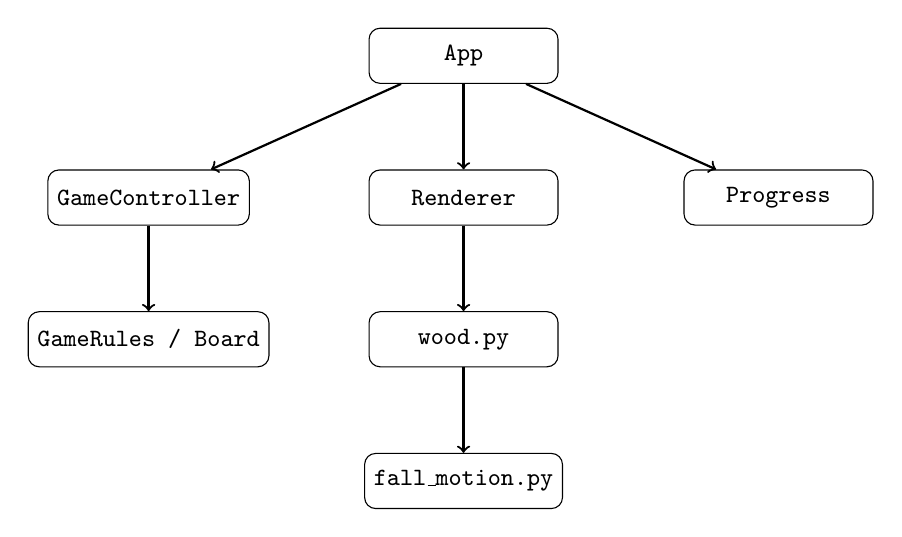
\begin{tikzpicture}[
        box/.style={draw, rounded corners, minimum height=0.7cm,
                    minimum width=2.4cm, align=center, font=\small},
        edge/.style={->, thick}
    ]
        \node[box] (app) at (0,0) {\texttt{App}};
        \node[box] (controller) at (-4,-1.8) {\texttt{GameController}};
        \node[box] (renderer) at (0,-1.8) {\texttt{Renderer}};
        \node[box] (progress) at (4,-1.8) {\texttt{Progress}};
        \node[box] (rules) at (-4,-3.6) {\texttt{GameRules / Board}};
        \node[box] (wood) at (0,-3.6) {\texttt{wood.py}};
        \node[box] (fall) at (0,-5.4) {\texttt{fall\_motion.py}};

        \draw[edge] (app) -- (controller);
        \draw[edge] (app) -- (renderer);
        \draw[edge] (app) -- (progress);
        \draw[edge] (controller) -- (rules);
        \draw[edge] (renderer) -- (wood);
        \draw[edge] (wood) -- (fall);
    \end{tikzpicture}
    \caption{Quan hệ sử dụng giữa các module của FrontEnd.}
    \label{fig:frontend_modules}
\end{figure}

Dữ liệu đi theo một chiều: \texttt{BackEnd} sinh \texttt{GameState} mới
sau mỗi hành động, \texttt{GameController} lưu lại trạng thái đó, còn
\texttt{Renderer}/\texttt{wood.py} chỉ đọc trạng thái và tham số hoạt ảnh
để vẽ, không module FrontEnd nào chỉnh sửa trực tiếp \texttt{Board} hay
\texttt{GameRules} ngoài thông qua \texttt{GameController}. Nhờ vậy chơi
thủ công, hiển thị lại lời giải và vẽ lại khung hình khi đổi kích thước cửa
sổ đều dùng chung một nguồn trạng thái duy nhất.

\subsection{Thiết kế các lớp chính}

Các lớp của FrontEnd được tổ chức theo quan hệ
\textit{composition}: mỗi lớp chỉ giữ tham chiếu tới đối tượng cần dùng
chứ không sao chép trạng thái, tránh lệch dữ liệu giữa giao diện và bộ
luật.
\begin{itemize}
    \item \texttt{GameController} đóng gói một \texttt{Board} và \texttt{GameRules}
    cho một màn chơi, đồng thời lưu \texttt{history} (các cặp trạng thái-hành
    động đã thực hiện) phục vụ hiển thị số bước và chơi lại màn.
    \item Hàm \texttt{move(action)} gọi \texttt{GameRules.apply\_action()}; nếu kết quả
    là \texttt{None} thì trạng thái được đánh dấu \texttt{"lost"}, ngược lại
    trạng thái mới được ghi vào \texttt{Board} và kiểm tra đích bằng
    \texttt{GameRules.is\_goal()}. Vì chơi thủ công và phát lại lời giải đều
    đi qua cùng hàm này, hành vi luôn khớp với bộ luật dùng trong tìm kiếm.
    \item Tham số \texttt{replay} phân biệt hai luồng gọi: khi \texttt{replay=False}
    (người chơi tự di chuyển), lời giải và kết quả benchmark cũ bị xóa qua
    \texttt{clear\_solution()} vì chúng không còn khớp với trạng thái hiện tại;
    khi \texttt{replay=True}, lịch sử tìm kiếm được giữ nguyên.
    \item Các hàm \texttt{set\_solution()}, \texttt{start\_replay()} và
    \texttt{step()} phục vụ riêng cho luồng phát lại lời giải, được mô tả
    chi tiết ở Mục~\ref{sec:ui_solver}.
    \item \texttt{Renderer} không giữ trạng thái trò chơi: mọi lời gọi vẽ nhận
    \texttt{state} và tham số hoạt ảnh làm đầu vào, nên cùng một lớp có thể vẽ
    cả khi chơi thủ công, khi phát lại và khi chỉ xem lại một khung hình tĩnh.
    \item \texttt{Progress} tách biệt hoàn toàn khỏi logic trò chơi, chỉ nhận
    tên màn và số bước để tính sao và lưu tiến độ xuống đĩa, nên không phụ thuộc
    \texttt{GameRules} và không bị ảnh hưởng nếu luật chơi thay đổi.
\end{itemize}

\subsection{Các cơ chế dựng hình và hoạt ảnh}
\label{sec:frontend_render}

\begin{description}
    \item[Phép chiếu isometric] \texttt{Renderer.board()} chiếu tọa độ
    lưới $(x,y,z)$ sang tọa độ màn hình bằng
    \[
        (u,v) = \big(o_x + (x-y)\cdot s,\; o_y + (x+y)\cdot s/2 - z\cdot s\big),
    \]
    với tỉ lệ $s$ tính để bàn chơi luôn vừa khung hiển thị và gốc chiếu
    $(o_x,o_y)$ đặt tại tâm khung.

    \item[Vẽ ô (\texttt{prism()})] Mỗi ô được vẽ bằng một hình hộp thấp,
    tô màu theo loại ô: nền, ô dễ vỡ (cam), cầu (nâu, gạch chéo đỏ khi
    đóng) và công tắc (vòng tròn \texttt{O}/\texttt{X}/hai chấm tương ứng
    \texttt{SoftSwitch}/\texttt{HeavySwitch}/\texttt{SplitSwitch}). Cầu
    đang đóng được bỏ qua khi vẽ nhưng vẫn vẽ ô nền dưới cầu, vì
    \texttt{Board} cho phép cầu phủ lên một ô khác; trạng thái cầu dùng
    để vẽ là trạng thái \textit{trước} khi hoạt ảnh lăn bắt đầu, để cầu
    không đổi trạng thái giữa lúc khối đang lăn qua.

    \item[Hoạt ảnh lăn (\texttt{wood.py})] Khối xoay quanh cạnh tiếp đất
    theo hướng di chuyển (tham số \texttt{pivot}), với góc xoay
    $\theta(t) = \mathrm{smoothstep}(t)\cdot\pi/2$, $t\in[0,1]$ theo thời
    gian lăn (tối đa 0.28s hoặc theo tốc độ phát lại), trong đó
    \textit{smoothstep} là $t^2(3-2t)$. Khi thắng, khối hạ thấp dần và
    các mặt bị cắt tại $z=0$ (\texttt{clip\_floor}) để không hiển thị
    phần khối chìm dưới sàn.

    \item[Hoạt ảnh rơi (\texttt{fall\_motion.py})] \texttt{GameRules} chỉ
    trả \texttt{None} cho hành động khiến khối rơi, không giữ lại trạng
    thái trung gian để vẽ. \texttt{prepare\_fall()} tính lại cục bộ, chỉ
    phục vụ hiển thị: áp dụng phần xoay của hành động
    (\texttt{rules.\_roll()}) để suy ra vị trí "định đáp", xác định vị
    trí còn được đỡ (\texttt{supported}) và ô dễ vỡ bị vỡ
    (\texttt{broken}); nếu còn đúng một điểm tựa, cạnh lật được xác định
    làm trục xoay. \texttt{fall\_vertex()} dựng chuyển động hai giai
    đoạn: lật quanh cạnh đỡ trong $0.36$s đầu, sau đó rơi tự do với gia
    tốc không đổi ($z \mathrel{-}= 2.5t + 15t^2$), khối mờ dần ở cuối
    hoạt ảnh.

    \item[Hoạt ảnh sao (\texttt{draw\_victory()})] Độc lập với khối 3D:
    ba ngôi sao bật ra lệch nhau $0.12$s mỗi sao, phóng to theo hàm
    \textit{ease-out-back}
    \[
        f(t) = 1 + c_3(t-1)^3 + c_1(t-1)^2, \qquad c_1 = 1.70158,\ c_3 = c_1+1,
    \]
    tạo hiệu ứng vượt quá kích thước đích rồi co lại, khác với
    \textit{smoothstep} êm dùng cho khối gỗ. Số sao đạt được tô vàng, số
    còn lại tô xám.
\end{description}

\subsection{Luồng xử lý và tiến trình chơi}

Vòng lặp chính trong \texttt{App.run()} lần lượt: xử lý sự kiện bàn
phím/chuột, cập nhật tiến trình tìm kiếm đang chạy nếu có, tự động phát bước kế tiếp khi đang ở chế độ
\textit{Replay}, rồi vẽ lại khung hình. Phím mũi tên/WASD ứng với bốn
hướng lăn trên bàn isometric (không trùng trục màn hình do góc chiếu),
\texttt{Space} đổi khối con khi đã tách, \texttt{R} khởi động lại màn,
\texttt{Esc} hủy tìm kiếm hoặc đóng panel đang mở theo thứ tự ưu tiên. Mỗi
di chuyển hợp lệ hoặc không hợp lệ đều tạo một bản ghi \texttt{animation}
dùng chung bởi \texttt{Renderer} và \texttt{wood.py} để phát đúng hoạt ảnh
tương ứng.

Khi \texttt{GameController} báo trạng thái \texttt{"won"} ở chế độ chơi
thủ công,  \texttt{App.check\_victory()} đợi hoạt ảnh kết thúc rồi gọi
\texttt{Progress.complete(map\_name, moves)}: số sao được tính bằng
\texttt{stars\_for()} so với số bước mục tiêu (\texttt{TARGETS}), bản ghi
tốt nhất được giữ lại và ghi xuống \path{.save/progress.json} theo mẫu
ghi-tạm-rồi-đổi-tên (\texttt{.tmp} rồi \texttt{replace()}) để tránh hỏng
file nếu chương trình bị tắt giữa lúc ghi. \texttt{unlocked(level)} yêu
cầu mọi màn có số thứ tự nhỏ hơn đã hoàn thành, tức mở khóa tuần tự theo
chiến dịch. Khi trạng thái \texttt{"lost"}, \texttt{App.check\_defeat()}
tự khởi động lại màn sau khi hoạt ảnh rơi phát xong, không cần người chơi
nhấn \texttt{R}.

Chế độ \textit{Solve by algorithm} dùng lại đúng \texttt{GameController}
và \texttt{Renderer} nói trên nhưng không gọi \texttt{check\_victory()}/
\texttt{Progress.complete()} trong lúc phát lại, để kết quả giải bằng
thuật toán không ghi sao hay mở khóa chiến dịch thay người chơi.
